\begin{frame}{Multiple regression}{Estimating the model coefficients}


\begin{itemize}
    \item Using \textit{residuals}, we define the \textbf{residual sum of squares}(RSS) as \pause

    \begin{align*}
      RSS &=  e_1^2 + e_2^2 + \cdots e_n^2   \\
          &= \sum_{i=1}^n (y_i - \hat{\beta}_0 - \hat{\beta}_1 x_{i1} -  \hat{\beta}_2 x_{i2} - \hat{\beta}_p x_{ip} )^2
    \end{align*}  \pause

    \item To estimate the coefficients we use the \textbf{least squares approach}, in which we seek to minimize RSS.  \pause

    \begin{columns}
         \column{0.50\linewidth}
         \hspace{0.5cm} $$ \hat{\beta} = (X'X)^{-1} X'y  $$  
           \column{0.50\linewidth}
            \centering
        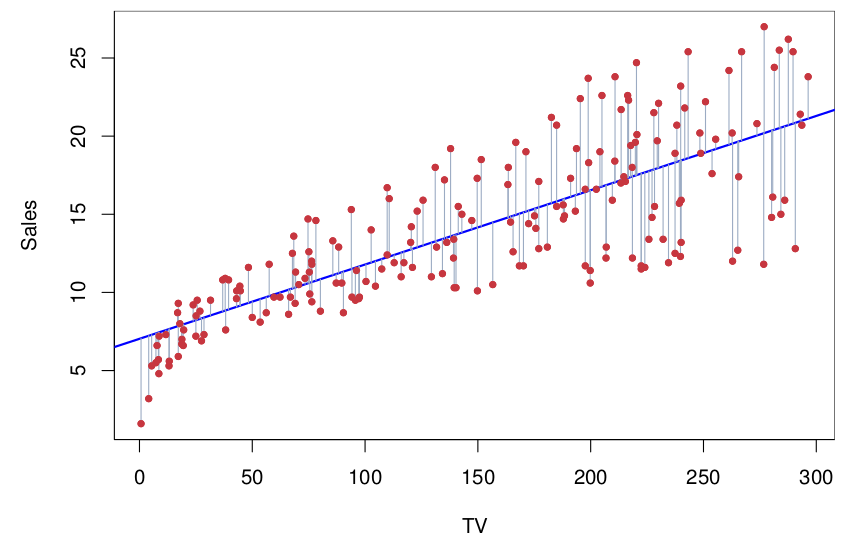
\includegraphics[height=4cm, width=4cm]{multiple-lr/ols.png}
    \end{columns} 

\end{itemize}

\end{frame}

